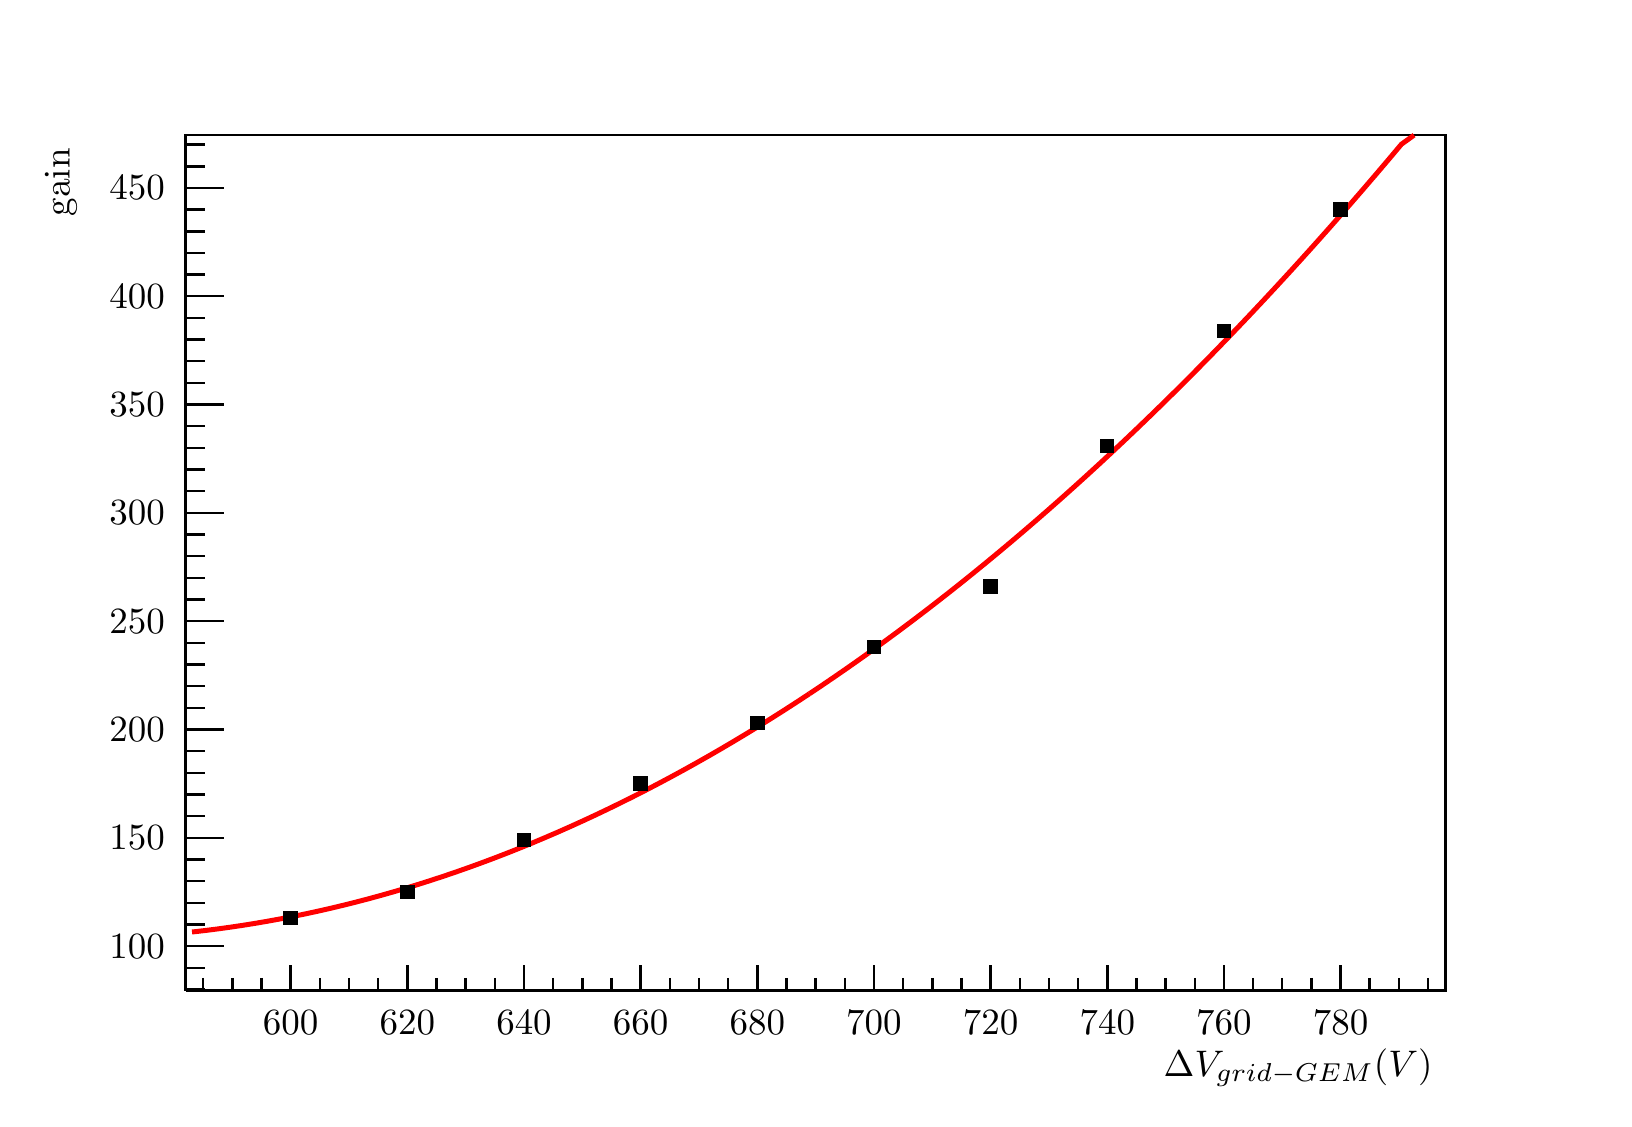
\begin{tikzpicture}
\pgfdeclareplotmark{cross} {
\pgfpathmoveto{\pgfpoint{-0.3\pgfplotmarksize}{\pgfplotmarksize}}
\pgfpathlineto{\pgfpoint{+0.3\pgfplotmarksize}{\pgfplotmarksize}}
\pgfpathlineto{\pgfpoint{+0.3\pgfplotmarksize}{0.3\pgfplotmarksize}}
\pgfpathlineto{\pgfpoint{+1\pgfplotmarksize}{0.3\pgfplotmarksize}}
\pgfpathlineto{\pgfpoint{+1\pgfplotmarksize}{-0.3\pgfplotmarksize}}
\pgfpathlineto{\pgfpoint{+0.3\pgfplotmarksize}{-0.3\pgfplotmarksize}}
\pgfpathlineto{\pgfpoint{+0.3\pgfplotmarksize}{-1.\pgfplotmarksize}}
\pgfpathlineto{\pgfpoint{-0.3\pgfplotmarksize}{-1.\pgfplotmarksize}}
\pgfpathlineto{\pgfpoint{-0.3\pgfplotmarksize}{-0.3\pgfplotmarksize}}
\pgfpathlineto{\pgfpoint{-1.\pgfplotmarksize}{-0.3\pgfplotmarksize}}
\pgfpathlineto{\pgfpoint{-1.\pgfplotmarksize}{0.3\pgfplotmarksize}}
\pgfpathlineto{\pgfpoint{-0.3\pgfplotmarksize}{0.3\pgfplotmarksize}}
\pgfpathclose
\pgfusepathqstroke
}
\pgfdeclareplotmark{cross*} {
\pgfpathmoveto{\pgfpoint{-0.3\pgfplotmarksize}{\pgfplotmarksize}}
\pgfpathlineto{\pgfpoint{+0.3\pgfplotmarksize}{\pgfplotmarksize}}
\pgfpathlineto{\pgfpoint{+0.3\pgfplotmarksize}{0.3\pgfplotmarksize}}
\pgfpathlineto{\pgfpoint{+1\pgfplotmarksize}{0.3\pgfplotmarksize}}
\pgfpathlineto{\pgfpoint{+1\pgfplotmarksize}{-0.3\pgfplotmarksize}}
\pgfpathlineto{\pgfpoint{+0.3\pgfplotmarksize}{-0.3\pgfplotmarksize}}
\pgfpathlineto{\pgfpoint{+0.3\pgfplotmarksize}{-1.\pgfplotmarksize}}
\pgfpathlineto{\pgfpoint{-0.3\pgfplotmarksize}{-1.\pgfplotmarksize}}
\pgfpathlineto{\pgfpoint{-0.3\pgfplotmarksize}{-0.3\pgfplotmarksize}}
\pgfpathlineto{\pgfpoint{-1.\pgfplotmarksize}{-0.3\pgfplotmarksize}}
\pgfpathlineto{\pgfpoint{-1.\pgfplotmarksize}{0.3\pgfplotmarksize}}
\pgfpathlineto{\pgfpoint{-0.3\pgfplotmarksize}{0.3\pgfplotmarksize}}
\pgfpathclose
\pgfusepathqfillstroke
}
\pgfdeclareplotmark{newstar} {
\pgfpathmoveto{\pgfqpoint{0pt}{\pgfplotmarksize}}
\pgfpathlineto{\pgfqpointpolar{44}{0.5\pgfplotmarksize}}
\pgfpathlineto{\pgfqpointpolar{18}{\pgfplotmarksize}}
\pgfpathlineto{\pgfqpointpolar{-20}{0.5\pgfplotmarksize}}
\pgfpathlineto{\pgfqpointpolar{-54}{\pgfplotmarksize}}
\pgfpathlineto{\pgfqpointpolar{-90}{0.5\pgfplotmarksize}}
\pgfpathlineto{\pgfqpointpolar{234}{\pgfplotmarksize}}
\pgfpathlineto{\pgfqpointpolar{198}{0.5\pgfplotmarksize}}
\pgfpathlineto{\pgfqpointpolar{162}{\pgfplotmarksize}}
\pgfpathlineto{\pgfqpointpolar{134}{0.5\pgfplotmarksize}}
\pgfpathclose
\pgfusepathqstroke
}
\pgfdeclareplotmark{newstar*} {
\pgfpathmoveto{\pgfqpoint{0pt}{\pgfplotmarksize}}
\pgfpathlineto{\pgfqpointpolar{44}{0.5\pgfplotmarksize}}
\pgfpathlineto{\pgfqpointpolar{18}{\pgfplotmarksize}}
\pgfpathlineto{\pgfqpointpolar{-20}{0.5\pgfplotmarksize}}
\pgfpathlineto{\pgfqpointpolar{-54}{\pgfplotmarksize}}
\pgfpathlineto{\pgfqpointpolar{-90}{0.5\pgfplotmarksize}}
\pgfpathlineto{\pgfqpointpolar{234}{\pgfplotmarksize}}
\pgfpathlineto{\pgfqpointpolar{198}{0.5\pgfplotmarksize}}
\pgfpathlineto{\pgfqpointpolar{162}{\pgfplotmarksize}}
\pgfpathlineto{\pgfqpointpolar{134}{0.5\pgfplotmarksize}}
\pgfpathclose
\pgfusepathqfillstroke
}
\definecolor{c}{rgb}{1,1,1};
\draw [color=c, fill=c] (0,0) rectangle (20,13.5817);
\draw [color=c, fill=c] (2,1.35817) rectangle (18,12.2235);
\definecolor{c}{rgb}{0,0,0};
\draw [c,line width=0.9] (2,1.35817) -- (2,12.2235) -- (18,12.2235) -- (18,1.35817) -- (2,1.35817);
\draw [c,line width=0.9] (2,1.35817) -- (18,1.35817);
\draw [c,line width=0.9] (3.33333,1.68413) -- (3.33333,1.35817);
\draw [c,line width=0.9] (3.7037,1.52115) -- (3.7037,1.35817);
\draw [c,line width=0.9] (4.07407,1.52115) -- (4.07407,1.35817);
\draw [c,line width=0.9] (4.44444,1.52115) -- (4.44444,1.35817);
\draw [c,line width=0.9] (4.81482,1.68413) -- (4.81482,1.35817);
\draw [c,line width=0.9] (5.18519,1.52115) -- (5.18519,1.35817);
\draw [c,line width=0.9] (5.55556,1.52115) -- (5.55556,1.35817);
\draw [c,line width=0.9] (5.92593,1.52115) -- (5.92593,1.35817);
\draw [c,line width=0.9] (6.2963,1.68413) -- (6.2963,1.35817);
\draw [c,line width=0.9] (6.66667,1.52115) -- (6.66667,1.35817);
\draw [c,line width=0.9] (7.03704,1.52115) -- (7.03704,1.35817);
\draw [c,line width=0.9] (7.40741,1.52115) -- (7.40741,1.35817);
\draw [c,line width=0.9] (7.77778,1.68413) -- (7.77778,1.35817);
\draw [c,line width=0.9] (8.14815,1.52115) -- (8.14815,1.35817);
\draw [c,line width=0.9] (8.51852,1.52115) -- (8.51852,1.35817);
\draw [c,line width=0.9] (8.88889,1.52115) -- (8.88889,1.35817);
\draw [c,line width=0.9] (9.25926,1.68413) -- (9.25926,1.35817);
\draw [c,line width=0.9] (9.62963,1.52115) -- (9.62963,1.35817);
\draw [c,line width=0.9] (10,1.52115) -- (10,1.35817);
\draw [c,line width=0.9] (10.3704,1.52115) -- (10.3704,1.35817);
\draw [c,line width=0.9] (10.7407,1.68413) -- (10.7407,1.35817);
\draw [c,line width=0.9] (11.1111,1.52115) -- (11.1111,1.35817);
\draw [c,line width=0.9] (11.4815,1.52115) -- (11.4815,1.35817);
\draw [c,line width=0.9] (11.8519,1.52115) -- (11.8519,1.35817);
\draw [c,line width=0.9] (12.2222,1.68413) -- (12.2222,1.35817);
\draw [c,line width=0.9] (12.5926,1.52115) -- (12.5926,1.35817);
\draw [c,line width=0.9] (12.963,1.52115) -- (12.963,1.35817);
\draw [c,line width=0.9] (13.3333,1.52115) -- (13.3333,1.35817);
\draw [c,line width=0.9] (13.7037,1.68413) -- (13.7037,1.35817);
\draw [c,line width=0.9] (14.0741,1.52115) -- (14.0741,1.35817);
\draw [c,line width=0.9] (14.4444,1.52115) -- (14.4444,1.35817);
\draw [c,line width=0.9] (14.8148,1.52115) -- (14.8148,1.35817);
\draw [c,line width=0.9] (15.1852,1.68413) -- (15.1852,1.35817);
\draw [c,line width=0.9] (15.5556,1.52115) -- (15.5556,1.35817);
\draw [c,line width=0.9] (15.9259,1.52115) -- (15.9259,1.35817);
\draw [c,line width=0.9] (16.2963,1.52115) -- (16.2963,1.35817);
\draw [c,line width=0.9] (16.6667,1.68413) -- (16.6667,1.35817);
\draw [c,line width=0.9] (3.33333,1.68413) -- (3.33333,1.35817);
\draw [c,line width=0.9] (2.96296,1.52115) -- (2.96296,1.35817);
\draw [c,line width=0.9] (2.59259,1.52115) -- (2.59259,1.35817);
\draw [c,line width=0.9] (2.22222,1.52115) -- (2.22222,1.35817);
\draw [c,line width=0.9] (16.6667,1.68413) -- (16.6667,1.35817);
\draw [c,line width=0.9] (17.037,1.52115) -- (17.037,1.35817);
\draw [c,line width=0.9] (17.4074,1.52115) -- (17.4074,1.35817);
\draw [c,line width=0.9] (17.7778,1.52115) -- (17.7778,1.35817);
\draw [anchor=base] (3.33333,0.801318) node[scale=1.3364, color=c, rotate=0]{600};
\draw [anchor=base] (4.81482,0.801318) node[scale=1.3364, color=c, rotate=0]{620};
\draw [anchor=base] (6.2963,0.801318) node[scale=1.3364, color=c, rotate=0]{640};
\draw [anchor=base] (7.77778,0.801318) node[scale=1.3364, color=c, rotate=0]{660};
\draw [anchor=base] (9.25926,0.801318) node[scale=1.3364, color=c, rotate=0]{680};
\draw [anchor=base] (10.7407,0.801318) node[scale=1.3364, color=c, rotate=0]{700};
\draw [anchor=base] (12.2222,0.801318) node[scale=1.3364, color=c, rotate=0]{720};
\draw [anchor=base] (13.7037,0.801318) node[scale=1.3364, color=c, rotate=0]{740};
\draw [anchor=base] (15.1852,0.801318) node[scale=1.3364, color=c, rotate=0]{760};
\draw [anchor=base] (16.6667,0.801318) node[scale=1.3364, color=c, rotate=0]{780};
\draw [anchor= east] (18,0.380287) node[scale=1.3364, color=c, rotate=0]{$\Delta V_{\text{grid-GEM}}\text{ (V)}$};
\draw [c,line width=0.9] (2,1.35817) -- (2,12.2235);
\draw [c,line width=0.9] (2.48,1.92486) -- (2,1.92486);
\draw [c,line width=0.9] (2.24,2.19995) -- (2,2.19995);
\draw [c,line width=0.9] (2.24,2.47505) -- (2,2.47505);
\draw [c,line width=0.9] (2.24,2.75015) -- (2,2.75015);
\draw [c,line width=0.9] (2.24,3.02524) -- (2,3.02524);
\draw [c,line width=0.9] (2.48,3.30034) -- (2,3.30034);
\draw [c,line width=0.9] (2.24,3.57544) -- (2,3.57544);
\draw [c,line width=0.9] (2.24,3.85054) -- (2,3.85054);
\draw [c,line width=0.9] (2.24,4.12563) -- (2,4.12563);
\draw [c,line width=0.9] (2.24,4.40073) -- (2,4.40073);
\draw [c,line width=0.9] (2.48,4.67583) -- (2,4.67583);
\draw [c,line width=0.9] (2.24,4.95093) -- (2,4.95093);
\draw [c,line width=0.9] (2.24,5.22602) -- (2,5.22602);
\draw [c,line width=0.9] (2.24,5.50112) -- (2,5.50112);
\draw [c,line width=0.9] (2.24,5.77622) -- (2,5.77622);
\draw [c,line width=0.9] (2.48,6.05131) -- (2,6.05131);
\draw [c,line width=0.9] (2.24,6.32641) -- (2,6.32641);
\draw [c,line width=0.9] (2.24,6.60151) -- (2,6.60151);
\draw [c,line width=0.9] (2.24,6.87661) -- (2,6.87661);
\draw [c,line width=0.9] (2.24,7.1517) -- (2,7.1517);
\draw [c,line width=0.9] (2.48,7.4268) -- (2,7.4268);
\draw [c,line width=0.9] (2.24,7.7019) -- (2,7.7019);
\draw [c,line width=0.9] (2.24,7.977) -- (2,7.977);
\draw [c,line width=0.9] (2.24,8.25209) -- (2,8.25209);
\draw [c,line width=0.9] (2.24,8.52719) -- (2,8.52719);
\draw [c,line width=0.9] (2.48,8.80229) -- (2,8.80229);
\draw [c,line width=0.9] (2.24,9.07738) -- (2,9.07738);
\draw [c,line width=0.9] (2.24,9.35248) -- (2,9.35248);
\draw [c,line width=0.9] (2.24,9.62758) -- (2,9.62758);
\draw [c,line width=0.9] (2.24,9.90268) -- (2,9.90268);
\draw [c,line width=0.9] (2.48,10.1778) -- (2,10.1778);
\draw [c,line width=0.9] (2.24,10.4529) -- (2,10.4529);
\draw [c,line width=0.9] (2.24,10.728) -- (2,10.728);
\draw [c,line width=0.9] (2.24,11.0031) -- (2,11.0031);
\draw [c,line width=0.9] (2.24,11.2782) -- (2,11.2782);
\draw [c,line width=0.9] (2.48,11.5533) -- (2,11.5533);
\draw [c,line width=0.9] (2.48,1.92486) -- (2,1.92486);
\draw [c,line width=0.9] (2.24,1.64976) -- (2,1.64976);
\draw [c,line width=0.9] (2.24,1.37466) -- (2,1.37466);
\draw [c,line width=0.9] (2.48,11.5533) -- (2,11.5533);
\draw [c,line width=0.9] (2.24,11.8284) -- (2,11.8284);
\draw [c,line width=0.9] (2.24,12.1035) -- (2,12.1035);
\draw [anchor= east] (1.9,1.92486) node[scale=1.3364, color=c, rotate=0]{100};
\draw [anchor= east] (1.9,3.30034) node[scale=1.3364, color=c, rotate=0]{150};
\draw [anchor= east] (1.9,4.67583) node[scale=1.3364, color=c, rotate=0]{200};
\draw [anchor= east] (1.9,6.05131) node[scale=1.3364, color=c, rotate=0]{250};
\draw [anchor= east] (1.9,7.4268) node[scale=1.3364, color=c, rotate=0]{300};
\draw [anchor= east] (1.9,8.80229) node[scale=1.3364, color=c, rotate=0]{350};
\draw [anchor= east] (1.9,10.1778) node[scale=1.3364, color=c, rotate=0]{400};
\draw [anchor= east] (1.9,11.5533) node[scale=1.3364, color=c, rotate=0]{450};
\draw [anchor= east] (0.416,12.2235) node[scale=1.3364, color=c, rotate=90]{gain};
\foreach \P in {(3.33333,2.28248), (4.81482,2.6126), (6.2963,3.27283), (7.77778,3.98809), (9.25926,4.75836), (10.7407,5.7212), (12.2222,6.49147), (13.7037,8.2796), (15.1852,9.73762), (16.6667,11.2782)}{\draw[mark options={color=c,fill=c},mark
 size=2.402402pt,mark=square*] plot coordinates {\P};}
\definecolor{c}{rgb}{1,0,0};
\draw [c,line width=1.8] (2.08,2.10345) -- (2.24,2.12181) -- (2.4,2.14197) -- (2.56,2.16395) -- (2.72,2.18773) -- (2.88,2.21331) -- (3.04,2.24071) -- (3.2,2.26991) -- (3.36,2.30093) -- (3.52,2.33374) -- (3.68,2.36837) -- (3.84,2.4048) -- (4,2.44305)
 -- (4.16,2.4831) -- (4.32,2.52495) -- (4.48,2.56862) -- (4.64,2.61409) -- (4.8,2.66137) -- (4.96,2.71046) -- (5.12,2.76136) -- (5.28,2.81406) -- (5.44,2.86857) -- (5.6,2.92489) -- (5.76,2.98302) -- (5.92,3.04295) -- (6.08,3.10469) -- (6.24,3.16824)
 -- (6.4,3.2336) -- (6.56,3.30076) -- (6.72,3.36974) -- (6.88,3.44052) -- (7.04,3.5131) -- (7.2,3.5875) -- (7.36,3.6637) -- (7.52,3.74171) -- (7.68,3.82153) -- (7.84,3.90316) -- (8,3.98659) -- (8.16,4.07184) -- (8.32,4.15889) -- (8.48,4.24774) --
 (8.64,4.33841) -- (8.8,4.43088) -- (8.96,4.52516) -- (9.12,4.62125) -- (9.28,4.71914) -- (9.44,4.81885) -- (9.6,4.92036) -- (9.76,5.02368) -- (9.92,5.1288);
\draw [c,line width=1.8] (9.92,5.1288) -- (10.08,5.23574) -- (10.24,5.34448) -- (10.4,5.45503) -- (10.56,5.56739) -- (10.72,5.68155) -- (10.88,5.79752) -- (11.04,5.91531) -- (11.2,6.03489) -- (11.36,6.15629) -- (11.52,6.27949) -- (11.68,6.4045) --
 (11.84,6.53132) -- (12,6.65995) -- (12.16,6.79038) -- (12.32,6.92262) -- (12.48,7.05667) -- (12.64,7.19253) -- (12.8,7.3302) -- (12.96,7.46967) -- (13.12,7.61095) -- (13.28,7.75404) -- (13.44,7.89893) -- (13.6,8.04564) -- (13.76,8.19415) --
 (13.92,8.34447) -- (14.08,8.49659) -- (14.24,8.65053) -- (14.4,8.80627) -- (14.56,8.96382) -- (14.72,9.12318) -- (14.88,9.28434) -- (15.04,9.44731) -- (15.2,9.61209) -- (15.36,9.77868) -- (15.52,9.94708) -- (15.68,10.1173) -- (15.84,10.2893) --
 (16,10.4631) -- (16.16,10.6387) -- (16.32,10.8162) -- (16.48,10.9954) -- (16.64,11.1765) -- (16.8,11.3593) -- (16.96,11.544) -- (17.12,11.7305) -- (17.28,11.9187) -- (17.44,12.1088) -- (17.6,12.2235);
\definecolor{c}{rgb}{0,0,0};
\foreach \P in {(3.33333,2.28248), (4.81482,2.6126), (6.2963,3.27283), (7.77778,3.98809), (9.25926,4.75836), (10.7407,5.7212), (12.2222,6.49147), (13.7037,8.2796), (15.1852,9.73762), (16.6667,11.2782)}{\draw[mark options={color=c,fill=c},mark
 size=2.402402pt,mark=square*] plot coordinates {\P};}
\end{tikzpicture}
